\documentclass[11pt,a4paper]{article}

% ==================================================
% Pakete
% ==================================================

\usepackage[utf8]{inputenc}
\usepackage[T1]{fontenc}
\usepackage[ngerman]{babel}

\usepackage[
    top=1.7cm,
    bottom=1.7cm,
    left=2.2cm,
    right=2.2cm
]{geometry}

\usepackage{graphicx}
\usepackage{svg}
\usepackage{booktabs}
\usepackage{tabularx}
\usepackage{array}
\usepackage{enumitem}
\usepackage{float}
\usepackage{microtype}
\usepackage{xcolor}
\usepackage{hyperref}

% ==================================================
% Formatierung
% ==================================================

\setlength{\parindent}{0pt}
\setlength{\parskip}{3pt}

\setlist[itemize]{
    noitemsep,
    topsep=1pt,
    leftmargin=1.5em
}

\setlist[enumerate]{
    noitemsep,
    topsep=1pt,
    leftmargin=1.7em
}

\hypersetup{
    colorlinks=true,
    linkcolor=black,
    urlcolor=blue,
    citecolor=black
}

\emergencystretch=2em

% ==================================================
% Angaben
% ==================================================

\newcommand{\projektname}{Uni Speedrun}
\newcommand{\matrikelnummer}{IU14173187}
\newcommand{\kurs}{DLBDSOOFPP01\_D}

% ==================================================
% Dokument
% ==================================================

\begin{document}

\begin{center}
    {\Large\textbf{Reflexions- und Entwurfsdokument: \projektname}}\\[2pt]
    {\large Objektorientierte und funktionale Programmierung mit Python}\\[4pt]
    Justus Wächter \hfill Matrikelnummer: \matrikelnummer\\
    Portfoliophase 2 \hfill Kurs: \kurs
\end{center}

\hrule
\vspace{0.2cm}

% ==================================================
\section{Ausgangslage und Ziel der Phase 2}

In der ersten Portfoliophase wurde für das Projekt
\glqq Uni Speedrun\grqq{} ein fachliches Konzept für ein lokales
Dashboard zur Studienfortschrittsplanung entwickelt. Im Mittelpunkt
stehen ein Studienplan, die darin enthaltenen Module sowie deren
Bearbeitungs- und Prüfungsstatus.

In Phase 2 wurde untersucht, wie dieses Modell mit Python umgesetzt
werden kann. Dabei ging es nicht nur darum, die Klassen technisch
nachzubauen, sondern auch darum, die fachlichen Verantwortlichkeiten,
Kapselung und Beziehungen der Klassen kritisch zu überprüfen. Die
Ergebnisse wurden anschließend in das UML-Modell und die geplante
Gesamtarchitektur übertragen.

% ==================================================
\section{Untersuchung objektorientierter Konzepte in Python}

Für die Untersuchung wurden die zentralen Fachbegriffe als Python-
Klassen modelliert. Das Fachmodell besteht nun aus den drei Entity-
Klassen \textit{Studienplan}, \textit{Modul} und
\textit{Prüfungsleistung} sowie der Enumeration \textit{Modulstatus}.
Damit wird die Prüfungsverwaltung bewusst von den eigentlichen
Moduldaten getrennt.

Der \textit{Studienplan} verwaltet die Module und berechnet unter
anderem Fortschritt und Zeitprognose. Ein \textit{Modul} beschreibt
Name, ECTS, Bearbeitungsdauer, Reihenfolge und Status. Eine
\textit{Prüfungsleistung} enthält die zugehörigen Prüfungsdaten wie
Titel, Datum, Note und Bestanden-Status.

Die ursprünglich betrachtete Klasse \textit{Studienziel} wurde nicht
ergänzt. Für den lokalen Single-User-Prototyp können Zielwerte direkt
im Studienplan verwaltet werden. Eine zusätzliche Klasse würde hier
keinen ausreichenden fachlichen Mehrwert liefern.

% --------------------------------------------------
\subsection{Klassen, Objekte und Kapselung}

Die Umsetzung zeigt eine Besonderheit von Python: Anders als
beispielsweise Java erzwingt Python keine echte private Sichtbarkeit.
Attribute werden daher mit einem führenden Unterstrich gekennzeichnet,
beispielsweise \texttt{\_ects}. Die eigentliche fachliche Kapselung
erfolgt zusätzlich über \texttt{@property} und validierende Setter.

Diese Entscheidung ist insbesondere für Werte wie ECTS, Dauer und
Noten relevant. Eine Validierung ausschließlich im Konstruktor wäre
nicht ausreichend, weil ein Attribut danach erneut verändert werden
könnte. Deshalb prüfen die Setter auch spätere Änderungen. So kann
beispielsweise verhindert werden, dass ein negativer ECTS-Wert oder
eine ungültige Note gespeichert wird.

Die Tests prüfen sowohl die Erzeugung gültiger Objekte als auch die
Ablehnung ungültiger Werte. Zusätzlich werden Berechnungen des
Studienplans und die Verwaltung mehrerer Module überprüft.

\textbf{Ergebnis:} Die Python-Umsetzung bestätigt, dass die fachlichen
Regeln nicht nur bei der Objekterzeugung, sondern über den gesamten
Lebenszyklus eines Objekts geschützt werden müssen. Dies wurde bei der
Überarbeitung des UML-Modells berücksichtigt.
\newpage
% --------------------------------------------------
\subsection{Enumeration und Zustandsverwaltung}

Für den Modulstatus wird eine Enumeration verwendet. Zulässige
Zustände sind:

\begin{center}
\texttt{GEPLANT} \quad
\texttt{AKTIV} \quad
\texttt{WARTE\_AUF\_ERGEBNIS} \quad
\texttt{ABGESCHLOSSEN}
\end{center}

Die Enumeration verhindert beliebige Statuswerte. Die Zustandswechsel
werden über fachliche Methoden ausgelöst und nicht durch beliebige
String-Zuweisungen.

Der Zustand \texttt{WARTE\_AUF\_ERGEBNIS} wurde bewusst beibehalten.
Nach einer Prüfung kann ein Modul auf die Bewertung warten, während
das nächste Modul bereits geplant oder begonnen wird. Dadurch bildet
das Modell den tatsächlichen Ablauf des Studienverlaufs besser ab.

Die Tests prüfen sowohl gültige als auch unzulässige
Statusänderungen. Die Enumeration wurde deshalb im UML-Modell als
eigene Enumeration beibehalten.

% --------------------------------------------------
\subsection{Komposition und fachliche Beziehungen}

Die Beziehung zwischen \textit{Studienplan} und \textit{Modul} wird
fachlich als Komposition modelliert. Technisch enthält der
Studienplan zwar lediglich eine Python-Liste mit Objektreferenzen,
dies allein entscheidet jedoch noch nicht über Komposition oder
Aggregation.

Entscheidend ist die fachliche Lebenszyklusabhängigkeit: Die Module
gehören zum konkreten Studienverlauf des Studienplans. Werden diese
Verlaufsdaten nicht mehr im entsprechenden Studienplan geführt,
verlieren sie ihre fachliche Bedeutung. Entsprechend wird die
Beziehung im UML als Komposition dargestellt.

Auch eine \textit{Prüfungsleistung} gehört fachlich zu genau einem
Modul und wird deshalb als Teil dieses Moduls modelliert.

Die Eigenschaft \texttt{reihenfolge} wird ebenfalls fachlich
begründet. Sie definiert die Reihenfolge der Module innerhalb des
Studienverlaufs und wird vom Domain-Modell für die zeitliche Planung
und Prognose verwendet. Die spätere SQLite-Speicherung übernimmt
diese Reihenfolge lediglich als Persistenzdetail.

Die Tests überprüfen das Hinzufügen mehrerer Module, die Sortierung
nach Reihenfolge und die Ermittlung des nächsten Moduls.

% --------------------------------------------------
\subsection{Vererbung und Abstraktion}

Für die drei Entity-Klassen wurde keine Vererbung eingesetzt, da
zwischen Studienplan, Modul und Prüfungsleistung keine sinnvolle
\glqq ist-ein\grqq-Beziehung besteht. Die unterschiedlichen
Modulzustände werden stattdessen durch die Enumeration
\textit{Modulstatus} abgebildet.

Vererbung wird dort eingesetzt, wo eine technische Abstraktion
sinnvoll ist. Das Repository wird über das Interface
\textit{StudienplanRepository} abstrahiert. Das konkrete
\textit{SQLiteStudienplanRepository} implementiert diese Schnittstelle
und übernimmt die relationale Speicherung.

Im UML wird diese Beziehung als korrekte Generalisierung dargestellt:
Eine durchgezogene Linie mit einer nicht ausgefüllten dreieckigen
Pfeilspitze zeigt von der konkreten Implementierung zur abstrakten
Oberklasse bzw. Schnittstelle.

% ==================================================
\subsection{Ergebnisse und Änderungen gegenüber Phase 1}

\begin{table}[H]
    \centering
    \scriptsize
    \caption{Wesentliche Änderungen gegenüber Phase 1}
    \begin{tabularx}{\textwidth}{
        >{\raggedright\arraybackslash}p{2.7cm}
        >{\raggedright\arraybackslash}p{2.8cm}
        >{\raggedright\arraybackslash}X
    }
        \toprule
        \textbf{Element} &
        \textbf{Entscheidung} &
        \textbf{Begründung} \\
        \midrule

        \textit{Studienplan} &
        beibehalten &
        Zentrales Planungsobjekt; verwaltet Module und berechnet
        Fortschritt sowie Zeitprognosen. \\

        \textit{Modul} &
        beibehalten und gekapselt &
        Fachliche Moduldaten werden über validierende Properties
        geschützt. \\

        \textit{Prüfungsleistung} &
        neu ergänzt &
        Prüfungsdaten werden von den eigentlichen Moduldaten getrennt
        und erhalten eine eigene Entity-Klasse. \\

        \textit{Modulstatus} &
        beibehalten &
        Begrenzte und kontrollierte Zustandsverwaltung. \\

        \textit{Studienziel} &
        nicht ergänzt &
        Für den lokalen Single-User-Prototyp reichen Zielwerte im
        Studienplan aus. \\

        \texttt{reihenfolge} &
        fachlich beibehalten &
        Definiert die Reihenfolge des Studienverlaufs und unterstützt
        die zeitliche Prognose. \\

        \bottomrule
    \end{tabularx}
\end{table}

% ==================================================
\section{Entwurf der Gesamtarchitektur}

\subsection{Architekturüberblick}

Die Gesamtarchitektur wird in vier Bereiche gegliedert, um
Benutzeroberfläche, Anwendungssteuerung, Fachmodell und Persistenz
voneinander zu trennen.

\begin{enumerate}
    \item
    \textbf{Fachmodell:}
    \textit{Studienplan}, \textit{Modul},
    \textit{Prüfungsleistung} und \textit{Modulstatus} enthalten die
    fachliche Logik und sind unabhängig von UI und SQL.

    \item
    \textbf{Controller:}
    Der \textit{DashboardController} koordiniert Benutzeraktionen,
    Zustandsänderungen und den Datenfluss zwischen UI, Fachmodell und
    Repository.

    \item
    \textbf{Persistenz:}
    Das Interface \textit{StudienplanRepository} definiert die
    benötigten Speicheroperationen. Das
    \textit{SQLiteStudienplanRepository} stellt die konkrete SQLite-
    Implementierung bereit.

    \item
    \textbf{Benutzeroberfläche:}
    \textit{DashboardScreen} ist für Darstellung und
    Benutzereingaben zuständig. \textit{UniSpeedrunApp} fungiert als
    Composition Root und erzeugt bzw. verbindet die benötigten
    Komponenten.
\end{enumerate}

% --------------------------------------------------
\subsection{UML-Klassendiagramm}

Das überarbeitete UML-Klassendiagramm bildet die fachliche und
technische Trennung ab. Im Fachmodell befinden sich die drei Entity-
Klassen und die Enumeration. Der Controller übernimmt die
Anwendungssteuerung, während das Repository die Persistenz kapselt.

\begin{figure}[H]
    \centering
    \IfFileExists{UML_PHASE2.svg}{
        \includesvg[
            width=0.88\textwidth,
            height=0.25\textheight,
            keepaspectratio,
            inkscapearea=drawing
        ]{UML_PHASE2}
    }{
        \IfFileExists{UML_PHASE2.png}{
            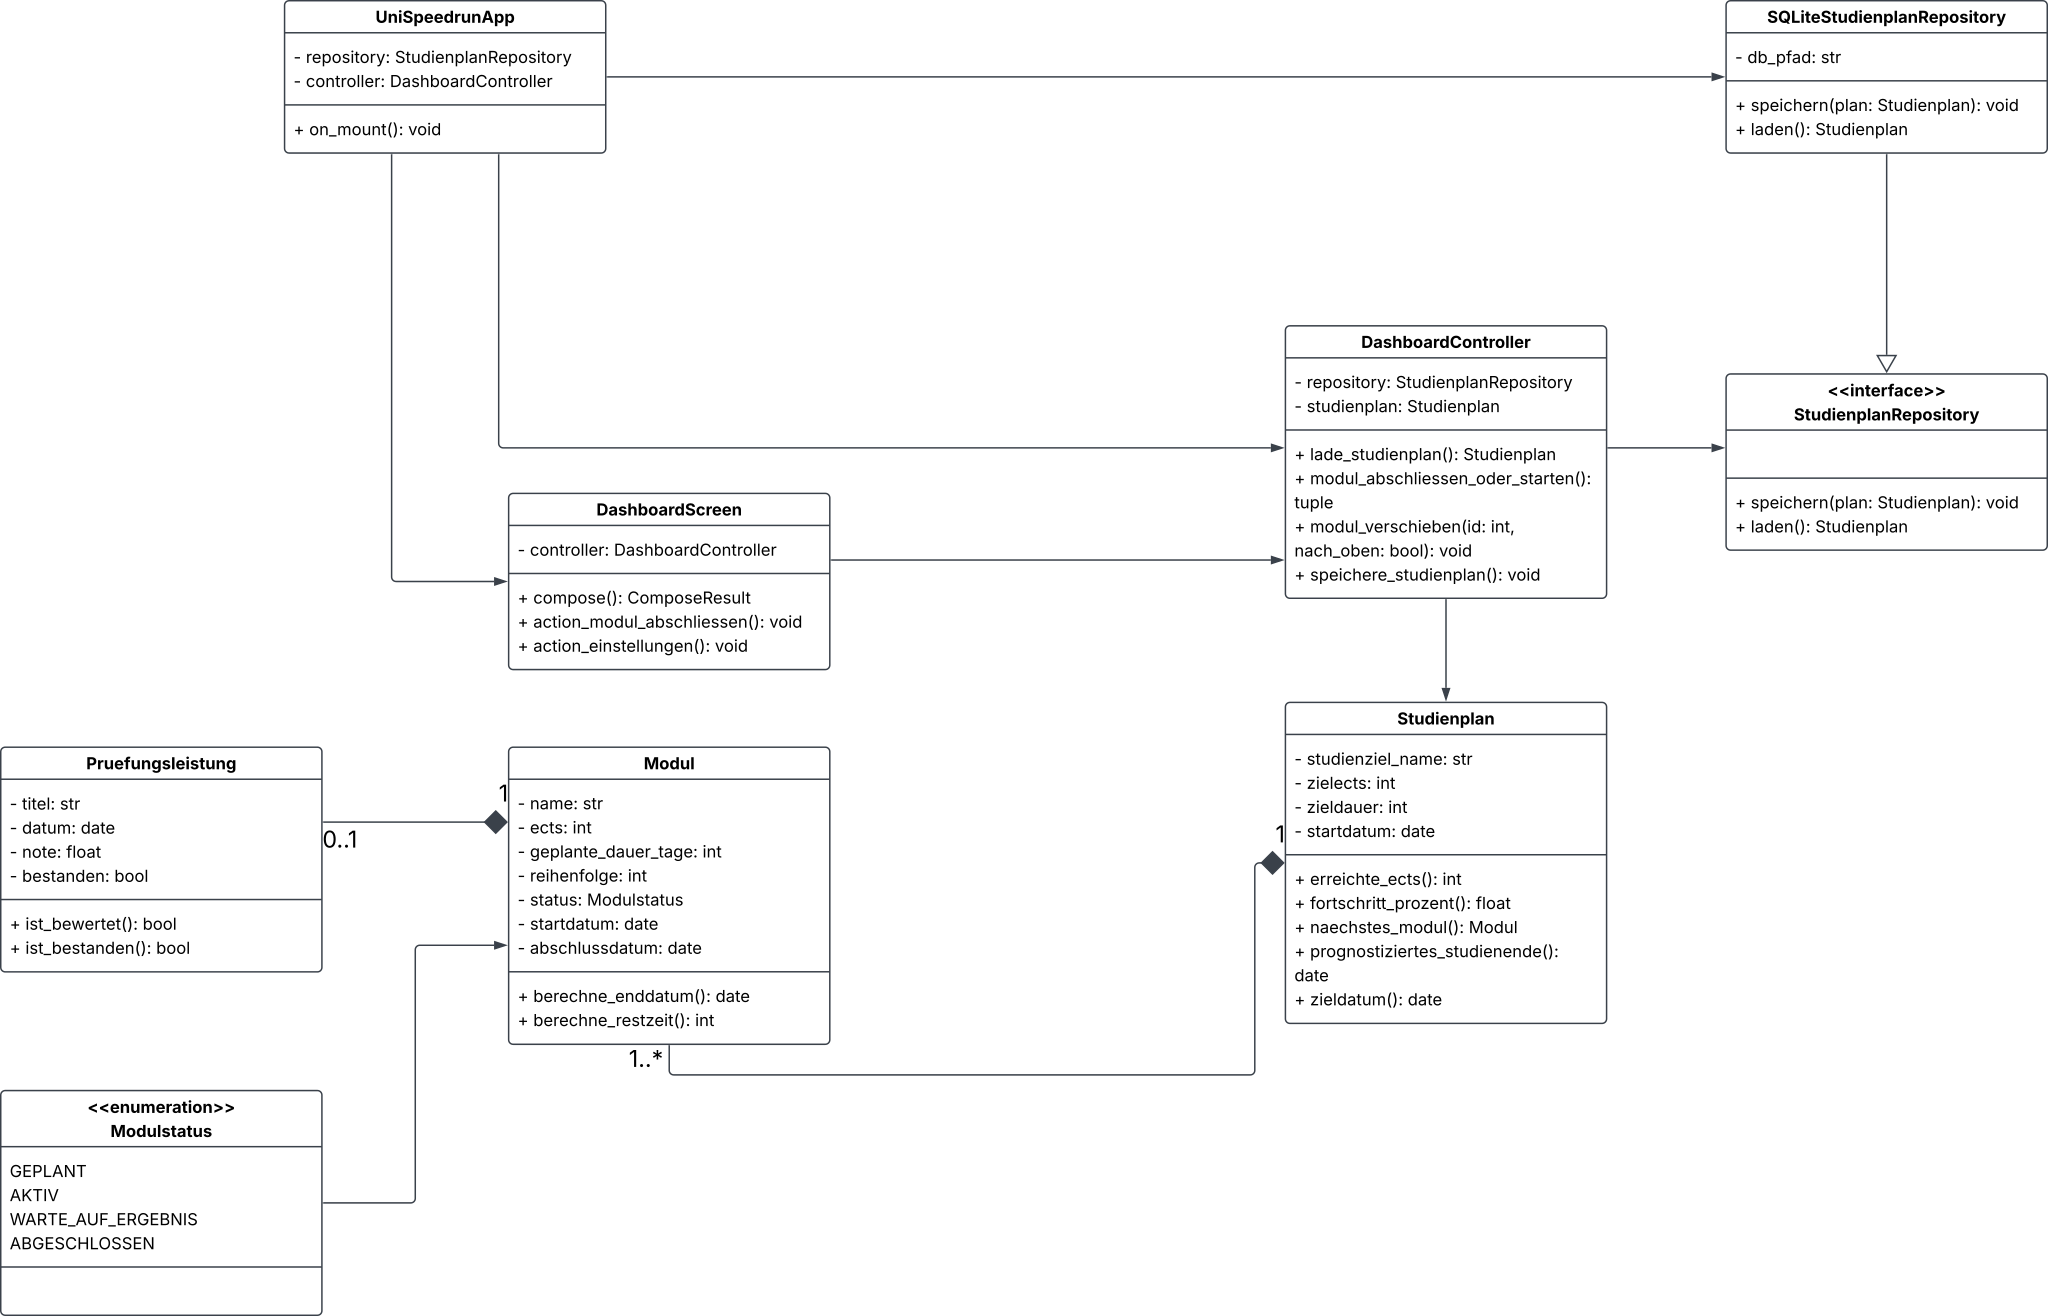
\includegraphics[
                width=0.88\textwidth,
                height=0.25\textheight,
                keepaspectratio
            ]{UML_PHASE2.png}
        }{
            \fbox{
                \parbox[c][4cm][c]{0.85\textwidth}{
                    \centering
                    UML-Klassendiagramm
                    \\[3pt]
                    \texttt{UML\_PHASE2.svg}
                }
            }
        }
    }
    \caption{UML-Klassendiagramm der Gesamtarchitektur, eigene Darstellung}
    \label{fig:gesamtarchitektur}
\end{figure}

% --------------------------------------------------
\subsection{Klassen und Verantwortlichkeiten}

\begin{table}[H]
    \centering
    \scriptsize
    \caption{Verantwortlichkeiten der Architektur}
    \begin{tabularx}{\textwidth}{
        >{\raggedright\arraybackslash}p{2.5cm}
        >{\raggedright\arraybackslash}p{3.2cm}
        >{\raggedright\arraybackslash}X
    }
        \toprule
        \textbf{Bereich} &
        \textbf{Klassen} &
        \textbf{Verantwortung} \\
        \midrule

        Fachmodell &
        Studienplan, Modul,
        Prüfungsleistung,
        Modulstatus &
        Fachliche Daten, Invarianten, Zustände und Berechnungen. \\

        Controller &
        DashboardController &
        Koordiniert Aktionen und verbindet UI, Fachmodell und
        Repository. \\

        UI &
        UniSpeedrunApp,
        DashboardScreen &
        Darstellung, Eingaben und Aufbau der Anwendung. \\

        Persistenz &
        StudienplanRepository,
        SQLiteStudienplanRepository &
        Abstraktion und konkrete Speicherung der Studienplandaten. \\

        \bottomrule
    \end{tabularx}
\end{table}

% --------------------------------------------------
\subsection{Zusammenarbeit der Komponenten}

Beim Start erzeugt \textit{UniSpeedrunApp} das konkrete Repository und
den \textit{DashboardController}. Das Repository wird per Dependency
Injection an den Controller übergeben. Dadurch muss weder der
\textit{DashboardScreen} noch das Fachmodell wissen, dass SQLite
verwendet wird.

Der \textit{DashboardScreen} stellt die Daten dar und nimmt
Benutzereingaben entgegen. Bei einer Aktion, beispielsweise dem
Abschluss eines Moduls, ruft der Screen den Controller auf. Der
Controller führt die entsprechende fachliche Operation aus und
veranlasst anschließend die Speicherung über das Repository.

Damit greift der Screen nicht direkt auf das Repository zu. Die
Verantwortung für die Anwendungssteuerung liegt beim Controller,
während das Fachmodell ausschließlich fachliche Regeln enthält.

Diese Trennung entspricht dem Prinzip der Separation of Concerns und
reduziert die Abhängigkeiten zwischen den einzelnen Bereichen.

% --------------------------------------------------
\subsection{Begründung der Architektur}

Die Einführung des \textit{DashboardController}s war eine direkte
Konsequenz aus der Überarbeitung gegenüber Phase 1. Zuvor enthielt
der DashboardScreen neben Darstellung auch Teile der
Anwendungssteuerung und hatte eine direkte Beziehung zum Repository.
Diese Verantwortlichkeiten werden nun getrennt.

Auch das Repository wird nicht direkt im Screen erzeugt. Die
Erzeugung der konkreten Komponenten erfolgt zentral durch
\textit{UniSpeedrunApp}. Dadurch ist klar definiert, wer für
Initialisierung und Dependency Injection verantwortlich ist.

SQLite wurde für den Prototyp gewählt, weil die Anwendung lokal und
für einen einzelnen Benutzer ausgelegt ist. Gleichzeitig erlaubt die
Repository-Abstraktion, später eine andere Persistenzlösung
einzuführen, ohne die fachlichen Klassen grundlegend zu verändern.

% ==================================================
\newpage
\section{Fazit und Vorbereitung der Implementierung}

Die Untersuchung hat gezeigt, dass das Fachmodell aus Phase 1 für die
Python-Umsetzung angepasst werden musste. Besonders relevant waren
die dauerhafte Kapselung fachlicher Werte, die Trennung der
Prüfungsverwaltung vom Modul und die klare Zuordnung der
Verantwortlichkeiten innerhalb der Gesamtarchitektur.

Mit
\textit{Studienplan},
\textit{Modul} und
\textit{Prüfungsleistung}
bestehen nun drei sinnvoll verbundene Entity-Klassen. Die
\textit{Modulstatus}-Enumeration kontrolliert den Lebenszyklus eines
Moduls. Validierende Properties stellen sicher, dass fachliche Regeln
auch bei späteren Änderungen eingehalten werden.

Gleichzeitig trennt der \textit{DashboardController} die
Anwendungssteuerung von der Darstellung. Das Repository kapselt die
Persistenz und wird über eine abstrakte Schnittstelle eingebunden.
Damit sind die wesentlichen Rückmeldungen aus Phase 2 in das Modell
eingeflossen.

Für Phase 3 bildet diese Architektur die Grundlage für die konkrete
Implementierung des Prototyps. Der Schwerpunkt liegt anschließend
darauf, die beschriebenen Klassen, Zustandsübergänge,
Persistenzoperationen und die Textual-Oberfläche tatsächlich
umzusetzen und durch weitere Tests zu überprüfen.

% ==================================================
\renewcommand{\refname}{Literatur- und Quellenverzeichnis}

\begin{thebibliography}{9}
\scriptsize

\bibitem{python-enum}
Python Software Foundation:
\textit{enum -- Support for enumerations}.
Online verfügbar unter:
\url{https://docs.python.org/3/library/enum.html},
abgerufen am 14.08.2026.

\bibitem{python-sqlite}
Python Software Foundation:
\textit{sqlite3 -- DB-API 2.0 interface for SQLite databases}.
Online verfügbar unter:
\url{https://docs.python.org/3/library/sqlite3.html},
abgerufen am 12.08.2026.

\bibitem{textual}
Textualize:
\textit{Textual Documentation}.
Online verfügbar unter:
\url{https://textual.textualize.io/},
abgerufen am 11.08.2026.

\bibitem{uml}
Object Management Group:
\textit{OMG Unified Modeling Language, Version 2.5.1}.
Online verfügbar unter:
\url{https://www.omg.org/spec/UML/2.5.1/PDF},
abgerufen am 14.08.2026.

\end{thebibliography}

\end{document}